\begin{frame}[fragile]
   \frametitle{Hello World Example}\scriptsize
\begin{itemize}
\item \texttt{hello.ci} file
   \begin{lstlisting}
mainmodule hello {
  mainchare Main {
    entry Main(CkArgMsg *m);
  };
};
   \end{lstlisting}
\item \texttt{hello.cpp} file
\lstset{basicstyle=\footnotesize}
   \begin{lstlisting}
#include <stdio.h>
#include "hello.decl.h"

class Main : public CBase_Main {
  public: Main(CkArgMsg* m) {
    ckout << "Hello World!" << endl;
    CkExit();
  };
};

#include "hello.def.h"
   \end{lstlisting}
\end{itemize}
\end{frame}

\begin{frame}[fragile]
   \frametitle{Hello World with Chares}\scriptsize
\begin{columns}
\begin{column}{.45\linewidth}
\texttt{hello.ci} file
   \begin{lstlisting}
mainmodule hello {
  mainchare Main { 
   entry Main(CkArgMsg *m); 
  };
  chare Singleton {
   entry Singleton();
  };
};
   \end{lstlisting}
\end{column}
\begin{column}{.55\linewidth}
\texttt{hello.cpp} file
\begin{lstlisting}
#include <stdio.h>
#include "hello.decl.h"

class Main : public CBase_Main {
  public: Main(CkArgMsg* m) {
    CProxy_Singleton::ckNew();
  };
};

class Singleton : public CBase_Singleton {
  public: Singleton() {
    ckout << "Hello World!" << endl;
    CkExit();
  };
};
#include "hello.def.h"
\end{lstlisting}
\end{column}
\end{columns}
\end{frame}


\subsection[Collections]{Object Collections}

% TODO: add picture of collections
\begin{frame}[fragile]
  \frametitle{Collections of Objects}
  \begin{itemize}
    \item Many problems have inherent order or structure
    \item Especially traditional `technical computing' problems
    \item Solution should use matching abstractions
    \item Arrays, lists, maps of parallel objects
    \item Specific segment of data, and associated computation and
      communication
    \item Need system support for efficient indexing
  \end{itemize}
\end{frame}

\begin{frame}[fragile]
  \frametitle{Collections of Objects: Concepts}
  \begin{itemize}
    \item Basic examples
      \begin{itemize}
      \item Matrix block
      \item Chunk of unstructured mesh
      \item Portion of distributed data structure
      \item Volume of simulation space
      \end{itemize}
      \pause
    \item Advanced Examples
      \begin{itemize}
      \item Abstract portions of computation
      \item Interactions among basic objects or underlying entities
      \end{itemize}
  \end{itemize}
\end{frame}

\begin{frame}[fragile]
  \frametitle{Collections of Objects}
  \begin{itemize}
    \item Structured: 1D, 2D, \ldots, 6D
    \item Unstructured: Anything hashable
      \pause
    \item Dense
    \item Sparse
      \pause
    \item Static - all created at once
    \item Dynamic - elements come and go
  \end{itemize}
\end{frame}

\begin{frame}[fragile]
  \frametitle{Collections of Objects: Communication}
  \begin{itemize}
    \item Point-to-point: to one element of a collection
    \item Broadcast: message to whole collection
    \item Multicast: message to subset of collection
    \item Reductions: message from (part of) collection
    \item Runtime system must provide efficient delivery for all
  \end{itemize}
\end{frame}

\begin{frame}[fragile]
  \frametitle{Collections of Objects: Runtime Service}
  \begin{itemize}
    \item System knows how to `find' objects efficiently: $(collection, index) \to processor$
    \item Applications can specify a mapping, or use simple
      runtime-provided options (e.g. blocked, round-robin)
    \item Distribution can be static, or dynamic!
    \item Key abstraction: application logic doesn't change, even
      though performance might
  \end{itemize}
\end{frame}

\begin{frame}[fragile]
  \frametitle{Collections of Objects: Runtime Service}
  \begin{itemize}
    \item Can develop and test logic in objects separately from their distribution
    \item Separation in time: make it work, then make it fast
    \item Division of labor: domain specialist writes object code, computationalist writes mapping
    \item Portability: different mappings for different systems, scales, or configurations
    \item Shared progress: improved mapping techniaues can benefit existing code
  \end{itemize}
\end{frame}




%% Object Collections: Supporting Data Decomposition (Phil)

%%     Motivate why object collections are needed
%%         simple adding numbers example
%%     Object Collections
%%         decompose data and associated work
%%         1/2/3D or more (eg: mesh chunk)
%%         dense / sparse (sparse solvers, collision detection)
%%         grow / shrink dynamically (AMR)
%%         each object exposes same functionality (methods)
%%         collection should be collectively addressable (method invocation on all objects)
%%         show sample pseudo-code snippets
%%     Object Collections: Collectives
%%     Examples
%%         simple scale a distributed vector (mcast)
%%         simple add array of numbers (mcast + redn)
%%         matrix vector product (mcast + gather)


\begin{frame}[fragile]
  \frametitle{Chare Array: Hello Example }
  \lstinputlisting{code/arrayHello.ci}
\end{frame}

\begin{frame}[fragile]
  \frametitle{Chare Array: Hello Example }
  \lstinputlisting[basicstyle=\scriptsize]{code/arrayHello.cpp}
\end{frame}

\begin{frame}[fragile]
   \frametitle{Hello World Array Projections Timeline View}\scriptsize
  \begin{itemize}
    \item ArrayHello on BG/Q 16 Nodes, mode c16, 1024 elements (4 per process)
  \end{itemize}
  \begin{center} 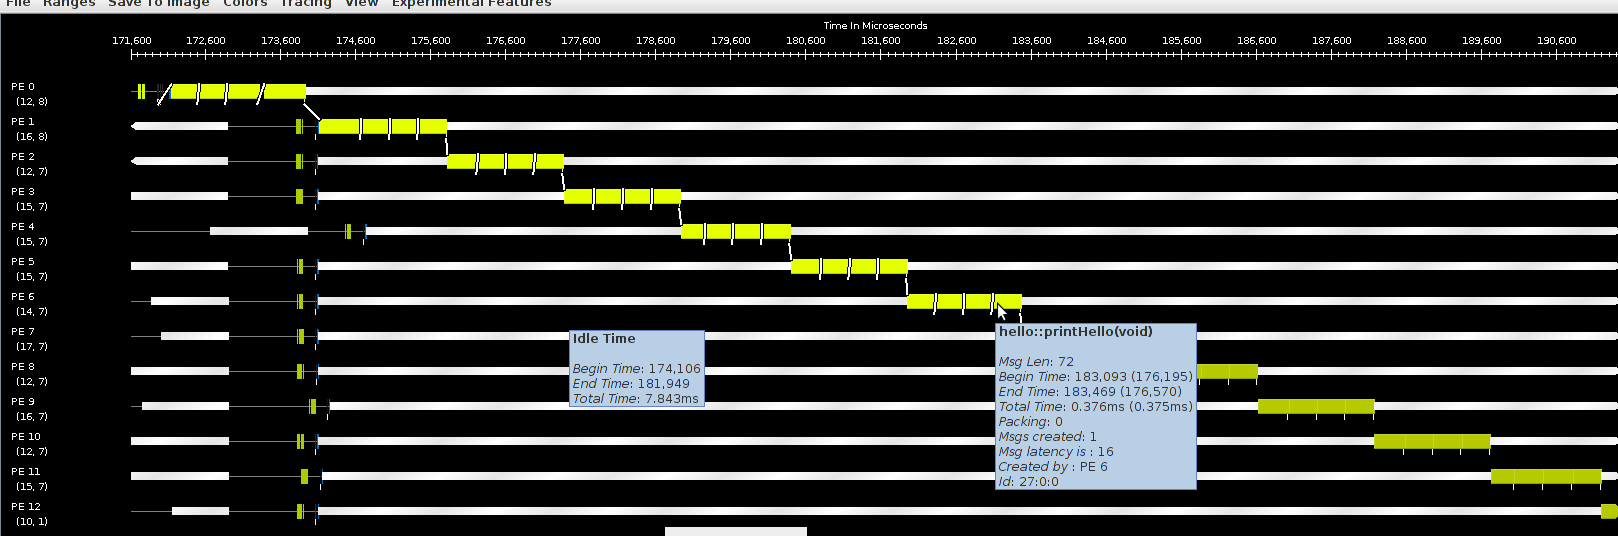
\includegraphics[width=0.99\textwidth]{figures/arrayHelloTimeline} \end{center}
\end{frame}


